
%*----------- SLIDE -------------------------------------------------------------
\begin{frame}[t]{Introdução} 
    \transdissolve[duration=0.5]

  	\begin{itemize}
        \item  Pong é o primeiro jogo eletrônico de sucesso da história, desenvolvido pela Atari Inc. e lançado no ano de 1972, iniciando uma febre de fliperamas.
        \item O jogo consiste na simulação de uma partida de tênis de mesa vista de cima, composta por uma bola, duas barras e o placar.
        \item O objetivo do jogo é fazer com que o oponente não consiga rebater a bola, somando pontos a medida que isso acontece.
    \end{itemize}
\vspace{0.3cm}
	\centering
	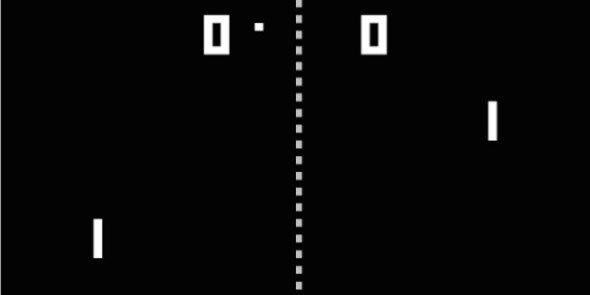
\includegraphics[width=0.4\textwidth]{pong-exemplo}    
          
%*----------- notes
    \note[item]{Notes can help you to remember important information. Turn on the notes option.}
\end{frame}
%-
%*----------- SLIDE -------------------------------------------------------------
\begin{frame}[c]{Introdução ao projeto}
 \transdissolve[duration=0.5]
 
\begin{itemize}
        \item  O projeto então tem em mente recriar o jogo Pong utilizando de tecnologias mais recentes.
        \item Para isso, será utilizada uma integração entre a linguagem de programação Processing e um microcontrolador
    \end{itemize}
\vspace{1cm}

\begin{columns}
	% Column 1
	\begin{column}{0.2\textwidth}
        	
\includegraphics[width=0.5\textwidth]{processing-logo} 
	\end{column}
	% Column 2    
		\begin{column}{0.2\textwidth}
		\centering
       	
\includegraphics[width=0.5\textwidth]{arduino-logo} 
	\end{column}
\end{columns}

%*----------- notes
    \note[item]{Notes can help you to remember important information. Turn on the notes option.}
\end{frame}
